\documentclass[10pt,aspectratio=169,hyperref={pdftex,unicode},xcolor=dvipsnames]{beamer}
\usepackage[english,russian]{babel}
\usepackage[utf8x]{inputenc}
\usepackage[T2A]{fontenc}
\usepackage{cmap}
\usepackage{paratype}
\newcommand{\mintedoptions}{outputdir=latexmk-build}
\usepackage[\mintedoptions]{minted}
\usepackage[normalem]{ulem} % для зачеркнутого текста
\usepackage{subcaption}
\usepackage{pgfplots}
\usepackage{pgfplotstable}
\usepackage{wrapfig}
\usepackage{fancyvrb}

\usetheme{metropolis}
\usefonttheme[]{professionalfonts}  % запрещаем beamer'у перезаписывать мат. шрифты
\metroset{numbering=none}
\metroset{subsectionpage=progressbar}

\hypersetup{
    colorlinks=true,
    linkcolor=blue,
    filecolor=magenta,
    urlcolor=cyan,
    pdfpagemode=FullScreen,
}

\setbeamercolor{frametitle}{fg=black}
\setbeamertemplate{frametitle}
{
 \vspace{3mm}\Large\insertframetitle\par\normalsize
}
\setbeamertemplate{title separator}{}
\setbeamertemplate{footnote separator}{}

\usetikzlibrary{shapes.geometric,arrows,fit,matrix,positioning}
\tikzset
{
    treenode/.style = {circle, draw=black, align=center, minimum size=1cm},
    subtree/.style  = {isosceles triangle, draw=black, align=center, minimum height=2cm, minimum width=2cm, shape border rotate=90, anchor=north}
}

\usebackgroundtemplate{\includegraphics[width=\paperwidth,height=\paperheight]{./common/background_white.jpg}}

\logo{\vspace{-0.7cm}\includegraphics[width=6mm]{./common/short-v.pdf}\hspace*{1.08\textwidth}}

\institute
{
  \begin{columns}
    \begin{column}{1.5cm}
    \includegraphics[height=15mm,keepaspectratio]{./common/math-cs.pdf}
    \end{column}
    \begin{column}{4cm}
          Факультет математики и компьютерных наук СПбГУ
    \end{column}
  \end{columns}
}

\begin{document}

\begin{frame}[plain]
  \begin{center}
    \textbf{ Андрей Хорохорин }

    { \Large\textbf{Разработка анализатора производительности программ по трассе исполнения с учётом микроархитектурных особенностей процессорного комплекса}}

    { Выпускная квалификационная работа }

    { \small Научный руководитель: Е.М. Линский }

    10.06.2025

  \end{center}


  \begin{columns}
    \begin{column}{1cm}
    \includegraphics[height=15mm,keepaspectratio]{./common/math-cs.pdf}
    \end{column}
    \begin{column}{10cm}
      \small
          Факультет математики и~компьютерных наук СПбГУ\\
          Программа <<Современное программирование>>
    \end{column}
  \end{columns}
\end{frame}

\usebackgroundtemplate{}
\setbeamertemplate{footline}[frame number]

\begin{frame}[fragile]{ Постановка задачи }
    При разработке производительных процессорных ядер для оценки полезности
    нововведений постоянно прибегают к измерению на бенчмарках.

    % Не всегда нововведение показывает лишь положительных эффект, в таких случаях
    % найти проблему бывает очень трудоёмко, а иногда и не возможно.

    % Сейчас для поиска проблемных мест наиболее пригодна трасса выполнения,
    % которая выглядит следующим образом:

    Пример HWT трассы:
\begin{verbatim}
< 5 > [00800051fc] lh      a4, 2(a4)        RD[0e]=000000000000000f
< 5 > [0080005200] bne     s9, a4, pc - 12
< 6 > [00800051f4] c.ld    a5, 0(a5)        RD[0f]=00000000800136b8
\end{verbatim}
    % Немного про hwt:
    % * проприетарная, кодируется аппаратурой без потери производительности
    % * привести скриншоты
    % * минимально влияет на динамику исполнения
    % * минусы:
    %     * доступна только на ПЛИС
    %     * сказать, что занимает много места

    Главная цель: облегчить анализ производительности и поиск проблемных мест
    при изменении как аппаратной, так и программной части.

    % Разработать инструмент для поиска проблемных с точки зрения производительности мест,
    % которые будут называться далее средством профилировки
    % Желательно с пояснением причины и место задержек.

    \begin{itemize}
        \pause \item подсказывать причину и место инцидента
        \pause \item возможность работать без ОС
        \pause \item учёт микроархитектурных особенностей при анализе
        \pause \item минимальные искажения динамики исполнения
        \pause \item удобство использования
    \end{itemize}
\end{frame}

\begin{frame}{ Обзор средств профилировки программ }
    \begin{itemize}
        \item
            HPM\textit{
                \footnotesize
                ~--- Hardware Performance Monitors (Аппаратные счётчики производительности)
            }
            \newline
                Пример: Perf, Intel V-Tune
        \item
            Сэмплирующие \newline
            Пример: Perf, Google Performance Tools
        \item
            Программные потактовые симуляторы \newline
            Пример: Gem5
    \end{itemize}

    % \only<1>{\vspace{\baselineskip}}
    \only<2>{ И всё не очень подходит в нашей ситуации! }

    % (для ускорения текст ниже читать не стоит)
    % HPM
    %   при работе с HPM необходимо заранее знать блок кода, на котором
    %   измеряются свойства программы. Поэтому на практике код может
    %   приходиться запустить до нескольких десятков раз.
    %   Частое считывание HPM влияет на динамику исполнения программы.
    % Сэмплирующие
    %   работают только под ОС
    %   не позволяют учесть микроархитектурные особенности для
    %   распознавания проблемы
    % Циклоточные эмуляторы
    %   решают проблему, но сложно поддерживать в актуальном состоянии
    %   предлагаемое решение чем-то похоже, но проще в реализации и поддержке

\end{frame}

\begin{frame}{ Общая схема решения }
    % * Идея: обрабатывать трассу поточно на хосте, подключенном к FPGA,
    %   который будет через PCIE получать HWT во время выполнения
    % * анализ должен работать достаточно быстро, чтобы не тормозить FPGA
    % * по возможности необходимо использовать минимум информации о микроархитектуре
    %   и максимум информации непосредственно из трассы.
    %   (чтобы при изменении небольших изменений в железе анализ не приходилось корректировать)
    % * бенчмарк должен запускаться один раз
    % * не требуется дополнительная инструментация кода
    \begin{center}
        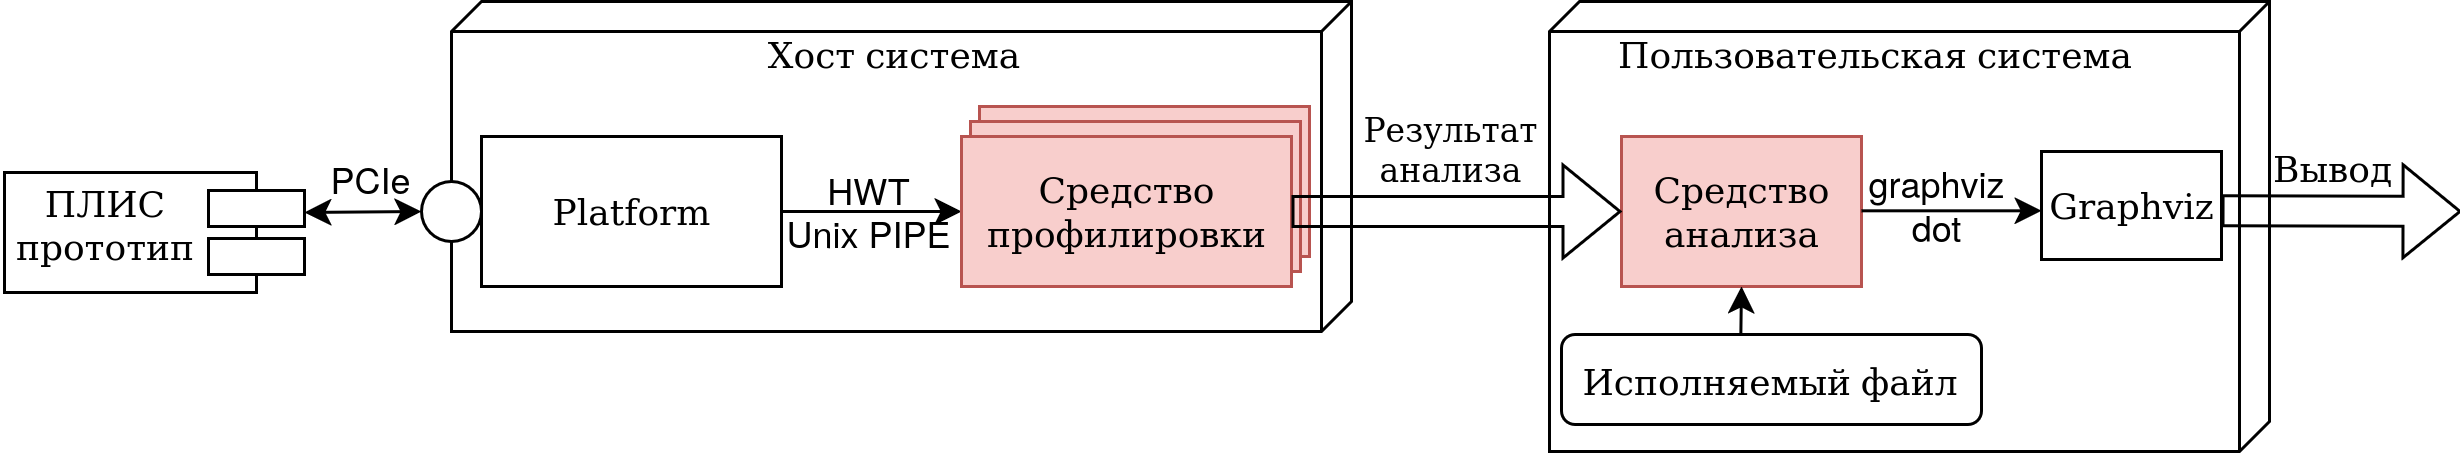
\includegraphics[width=\textwidth,keepaspectratio]{./images/stac_arch.png}
    \end{center}
    \begin{itemize}
        \pause \item анализ должен работать достаточно быстро, чтобы не тормозить FPGA
        \pause \item бенчмарк запускается один раз, трасса не записывается на диск
    \end{itemize}
\end{frame}

\begin{frame}{ Пример применения }
    Проблема: очки бенчмарка \href{https://github.com/eembc/coremark}{coremark}
    колеблются на $\sim2\%$ в зависимости от длины строки с флагами компиляции.
    % (согласитесь мало, но не приятно)
    % хочется понять, откуда такое поведение возникает.

    За основу возьмём два исполняемых файла (первый лучше второго).
    Запускаем для обоих средство профилировки, получая два файла с профилями исполнения.
\end{frame}

\begin{frame}{ Пример применения }
    Выводим статистику по функциям:
    \begin{figure}
        \begin{subfigure}{0.8\textwidth}
            \centering
            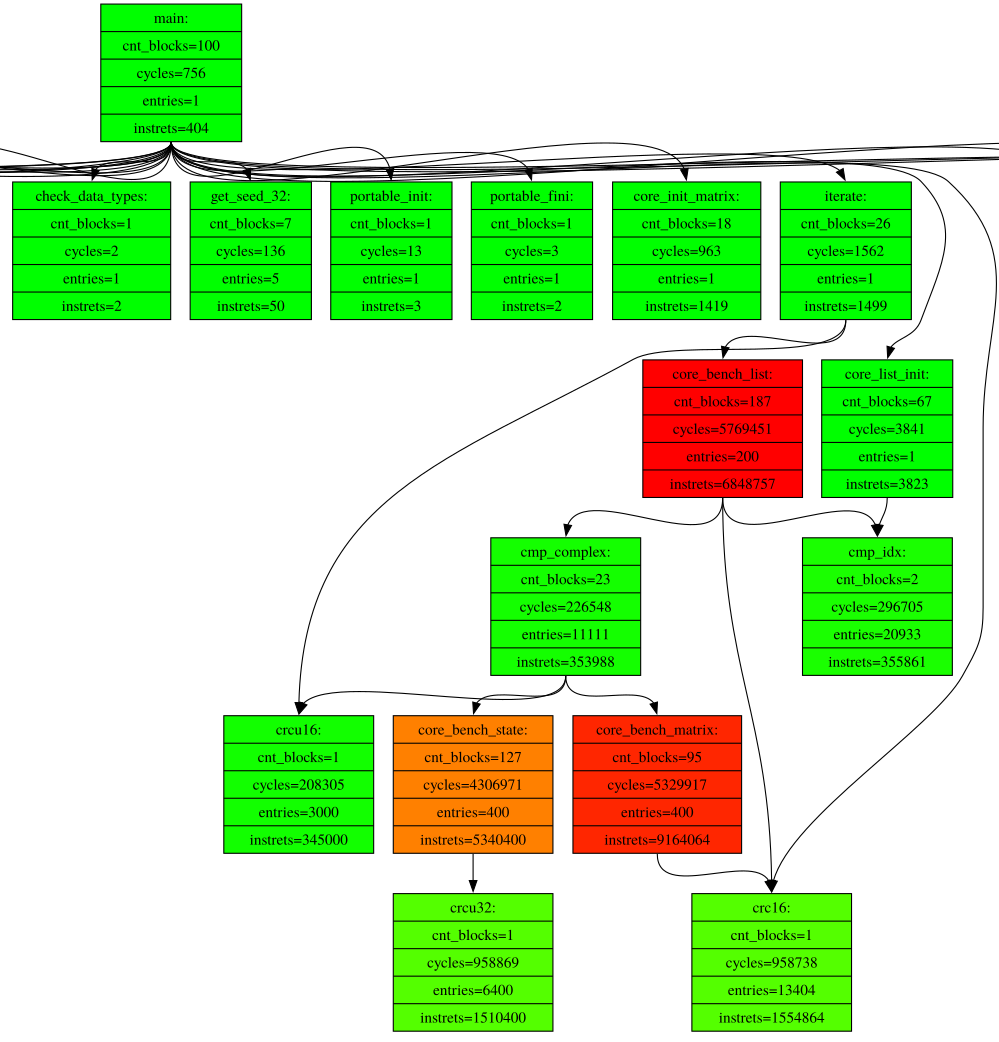
\includegraphics[height=0.8\textheight,keepaspectratio]{./images/stac_functions.png}
        \end{subfigure}
    \end{figure}

    % Справа можно увидеть основные метрики, необходимые для анализа производительности.
    % Любая задержка, распознаётся в одну из метрик, называние которой заканчивается на `_stall`
\end{frame}

\begin{frame}{ Пример применения }
    Сравнивать большое количество метрик на двух графах достаточно
    не удобно, поэтому можно воспользоваться режим для определения различий.

    % В этом режиме статистика базового (первого) запуска вычитается из второго.

    % Видно, что время выполнения второго варианта значительно отличается от первого
    % только в рамках одной функции.

    % Выдедем побольше метрик
    \begin{figure}
        \begin{subfigure}{0.45\textwidth}
            \centering
            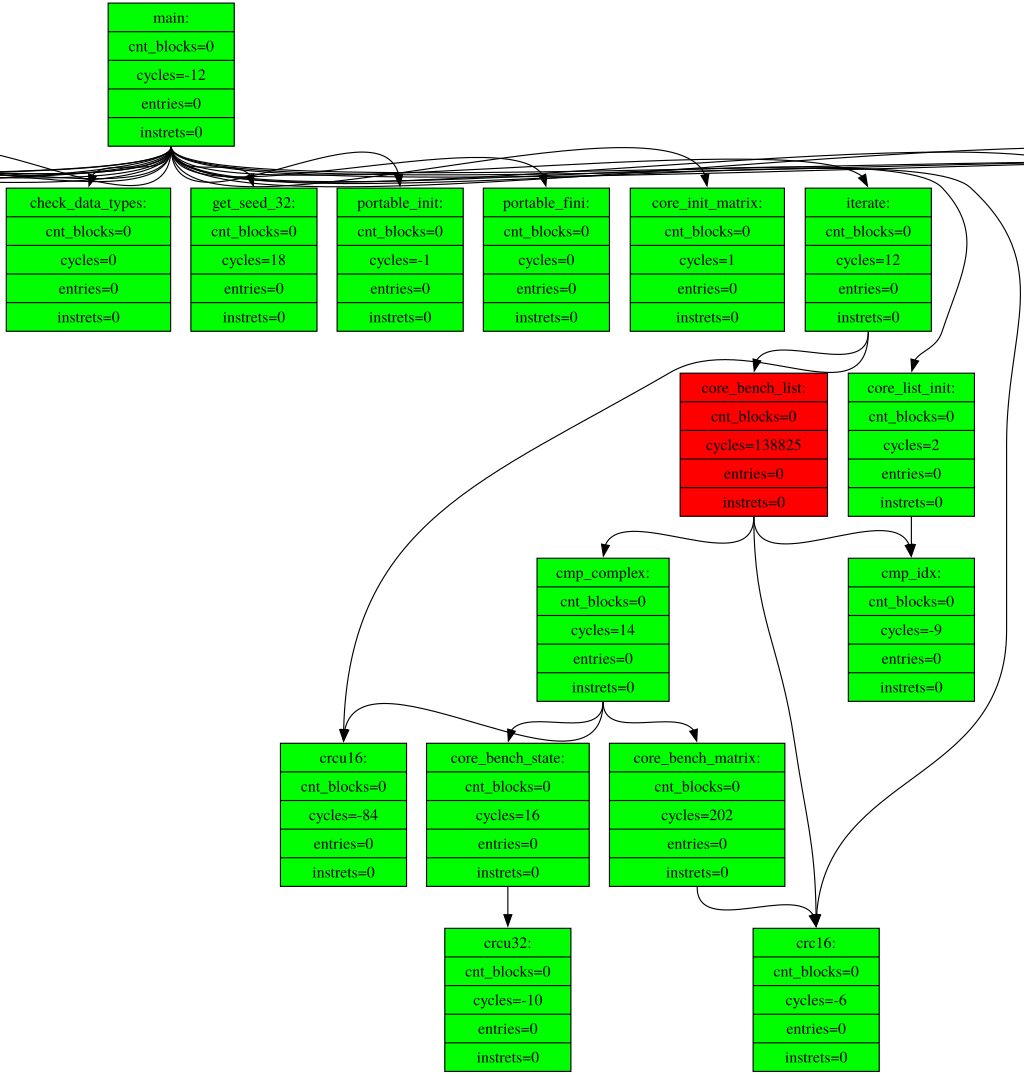
\includegraphics[height=0.7\textheight,keepaspectratio]{./images/stac_diff.png}
        \end{subfigure}
        \begin{subfigure}{0.45\textwidth}
            \centering
            \only<1>{\hspace{1cm}}
            \only<2>{
                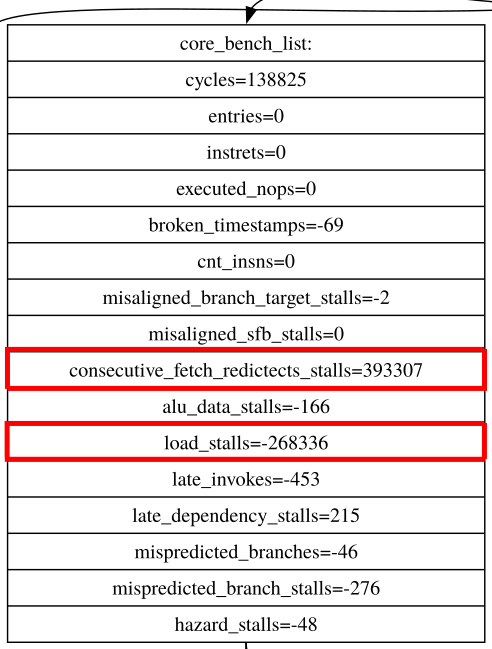
\includegraphics[height=0.7\textheight,keepaspectratio]{./images/stac_diff_zoom.png}
            }
        \end{subfigure}
    \end{figure}

    % Справа можно увидеть основные метрики, необходимые для анализа производительности.
    % Любая задержка, распознаётся в одну из метрик, называние которой заканчивается на `_stall`
\end{frame}

\begin{frame}[fragile]{ Сужаем область поиска }
    Выведем карту базовых блоков заданной функции.
    % раскрасив её по количеству увеличившихся задержек.

    % видим, что почти все задержки распределены в двух местах
    % на самом деле эти два места идентичны, поэтому рассмотрим только одно

\begin{SaveVerbatim}[]{VerbEnv}
800052f0:	ld a1, 8(a5)
800052f2:	lbu s6, 0(a1)
800052f6:	beq s7, s6, 80005204
800052fa:	ld a5, 0(a5)
800052fc:	bnez a5, 800052f0
\end{SaveVerbatim}

    \begin{figure}
        \begin{subfigure}{0.45\textwidth}
            \centering
            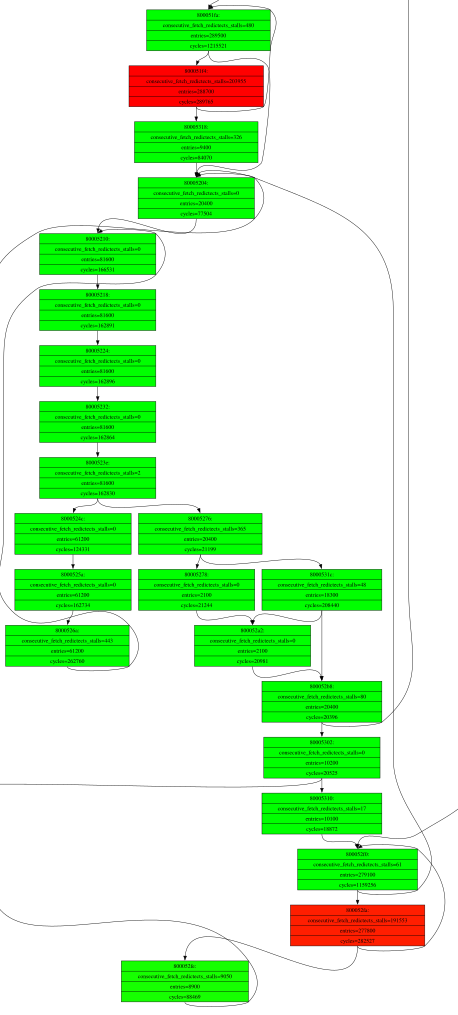
\includegraphics[height=0.8\textheight,keepaspectratio]{./images/stac_blocks.png}
        \end{subfigure}
        \begin{subfigure}{0.45\textwidth}
            \centering
            \only<1>{\hspace{1cm}}
            \only<2>{
                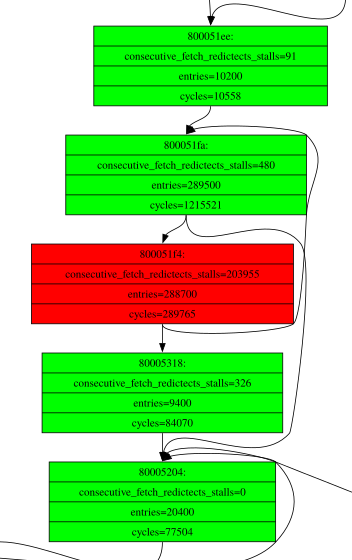
\includegraphics[height=4.5cm,keepaspectratio]{./images/stac_blocks_zoom.png}
                \newline

                \BUseVerbatim[fontshape=it,fontsize=\footnotesize,fontfamily=courier]{VerbEnv}
            }
        \end{subfigure}
    \end{figure}

    % Справа можно увидеть основные метрики, необходимые для анализа производительности.
    % Любая задержка, распознаётся в одну из метрик, называние которой заканчивается на `_stall`
\end{frame}

\begin{frame}{ Метрики }
    \begin{figure}
        \centering
        \includegraphics[height=0.8\textheight,keepaspectratio]{./images/stac_stalls.png}
    \end{figure}
\end{frame}

\begin{frame}[fragile]{ Пример: Late ALU }
    % Микроархитектурная особенность с строго очередным выполнением инструкций,
    % позволяющая спекулятивно отправить на выполнение инструкцию,
    % зависимость по данным которой ещё не готова.

\begin{figure}[h]
\centering
\begin{tikzpicture}[
    stage/.style={rectangle, draw, minimum width=1.5cm, minimum height=1cm},
    alu/.style={fill=green!20},
    arrow/.style={->, >=stealth}
]

% Рисуем стадии конвейера
\node[stage] (IF) at (0,0) {IF};
\node[stage,fill=violet!20] (ID) at (2,0) {ID};
\node[stage,alu] (ALU) at (4,0) {ALU};
\node[stage] (DC1) at (6,0) {DC-1};
\node[stage] (DC2) at (8,0) {DC-2};
\node[stage,alu] (LALU) at (10,0) {ALU};
\node[stage] (WB) at (12,0) {WB};

% Рисуем стрелки между стадиями
\draw[arrow] (IF) -- (ID);
\draw[arrow] (ID) -- (ALU);
\draw[arrow] (ALU) -- (DC1);
\draw[arrow] (DC1) -- (DC2);
\draw[arrow] (DC2) -- (LALU);
\draw[arrow] (LALU) -- (WB);

\draw[dashed, thick, arrow] (LALU) -- (10, -1) -- (4,-1) -- (ALU);

\end{tikzpicture}
\caption{Схема рассматриваемого конвейера}
\label{lalu}
\end{figure}

    Инструкция исполняется как \textit{late}, если:
    \begin{itemize}
        \item
            На момент начала исполнения существует неразрешённая зависимость по данным.
        \item
            Через 3 такта зависимость по данным \textit{почти точно} будет разрешена.
    \end{itemize}
\end{frame}

\begin{frame}[fragile]{ Пример: Late ALU }
\begin{minipage}[]{\linewidth}
    \begin{minipage}[]{0.5\linewidth}
    \begin{figure}[h]
        \centering
        \begin{minted}[fontsize=\footnotesize]{asm}
ld x1, addr1
ld x2, addr2
addi x1, x1, 1 (late)
addi x1, x1, 2 (late)
addi x1, x1, 3 (late)
addi x2, x2, 1
addi x2, x2, 2
addi x2, x2, 3
/* x1, x2 вычислено */
sd x1, addr1
sd x2, addr2
        \end{minted}
        \label{lalu_good_code}
        \caption{Код без задержек}
    \end{figure}
    \end{minipage}
    \begin{minipage}[]{0.50\linewidth}
    \begin{figure}[h]
        \centering
        \begin{minted}[fontsize=\footnotesize]{asm}
ld x1, addr1
ld x2, addr2
addi x1, x1, 1 (late)
addi x2, x2, 1 (late)
addi x1, x1, 2 (late)
addi x2, x2, 2 (late)
addi x1, x1, 3 (late)
addi x2, x2, 3 (late)
/* x1 и x2 будут вычислены через 3 такта */
sd x1, addr1
sd x2, addr2
        \end{minted}
        \label{lalu_bad_code}
        \caption{Код с задержкой}
    \end{figure}
    \end{minipage}
\end{minipage}
\end{frame}

\begin{frame}{ Архитектура разработанного средства }
    \begin{figure}
        \centering
        \includegraphics[height=0.8\textheight,keepaspectratio]{./images/stac_classes.png}
    \end{figure}
\end{frame}

\begin{frame}{ Результаты работы }
    В результате разработан инструмент, который:
    \begin{itemize}
        \item
        пригоден для поиска мест и причин снижения производительности
        % как увидели на разобранном примере
        \pause \item
        в большинстве сценариев способен обрабатывать данные
        без потери скорости выполнения на FPGA
        \pause \item
        требует лишь один запуск теста производительности для
        сбора всех метрик
        \pause \item
        значительно более точен, чем профилировка известными
        средствами
        \pause \item
        расширяем как в сторону добавления других микроархитектур,
        так и в сторону смены формата трассы.
    \end{itemize}
\end{frame}

\begin{frame}{ Спасибо за внимание! }
    Ссылка на репозиторий с работой: \href{https://github.com/khaser/stac}{github.com/khaser/stac}

    Ссылка на репозиторий со слайдами: \href{https://github.com/khaser/stac}{github.com/khaser/stac-report}

    % \begin{center}
    %     \includegraphics[height=0.6\textheight,keepaspectratio]{./images/stac_qr.png}
    %
    %     QR-код ссылки на репозиторий с работой
    % \end{center}
    \begin{figure}[h]
        \includegraphics[height=0.6\textheight,keepaspectratio]{./images/stac_qr.png}
        \caption{QR-код ссылки на репозиторий с работой}
        % \caption{Схема рассматриваемого конвейера}
        \label{qr}
    \end{figure}
\end{frame}

\begin{frame}{ Возможности для дальнейшей работы }
    \begin{itemize}
        \item поддержка трассировки процесса, запущенного под linux
        \item поддержка формата трассы, с большим количеством видимых стадий
              выполнения инструкций
        \item улучшения в user experience.
            \begin{itemize}
                \item переход на QT/GTK, интерактивность
                \item возможность вводить пользователькие метрики в виде формул над существующими.
            \end{itemize}
    \end{itemize}
\end{frame}

% \begin{frame}{ Ссылки на связанные работы }
% \begin{thebibliography}{9}
%
% \bibitem{intel_top_down}
% A Top-Down method for performance analysis and counters architecture (2014), Yasin, Ahmad
%
% doi:10.1109/ISPASS.2014.6844459
%
% \bibitem{riscv_spec}
% The RISC-V Instruction Set Manual Volume I: Unprivileged ISA, Version 20240411
%
% \end{thebibliography}
% \end{frame}

\end{document}
